\documentclass[11pt, a4paper]{article}
\usepackage[utf8]{inputenc}
\usepackage{fullpage}
\usepackage{amsmath,amsthm,amsfonts,amssymb,amscd}
\usepackage{lastpage}
\usepackage{enumerate}
\usepackage{fancyhdr}
\usepackage{mathrsfs}
\usepackage{xcolor}
\usepackage{graphicx}
\usepackage{listings}
\usepackage{preamble}
\usepackage{paralist}
\usepackage{ctable}
\usepackage{diagbox}
\usepackage{bm}
\usepackage{geometry}
\usepackage{float}
\usepackage{subfigure}
\usepackage{algorithm}
\usepackage{algorithmic}
\usepackage[colorlinks, linkcolor=blue]{hyperref}
\usepackage{animate}
\geometry{a4paper,scale=0.85}

\definecolor{codegreen}{rgb}{0,0.6,0}
\definecolor{codegray}{rgb}{0.5,0.5,0.5}
\definecolor{codepurple}{rgb}{0.58,0,0.82}
\definecolor{backcolour}{rgb}{0.95,0.95,0.92}

\lstdefinestyle{mystyle}{
    backgroundcolor=\color{backcolour},   
    commentstyle=\color{codegreen},
    keywordstyle=\color{magenta},
    numberstyle=\tiny\color{codegray},
    stringstyle=\color{codepurple},
    basicstyle=\ttfamily\footnotesize,
    breakatwhitespace=false,         
    breaklines=true,                 
    captionpos=b,                    
    keepspaces=true,                 
    numbers=left,                    
    numbersep=3pt,                  
    showspaces=false,                
    showstringspaces=false,
    showtabs=false,                  
    tabsize=2
}

\begin{document}

    \section{Numerical Solution of 2D Heat Equation Using PINN}
    \subsection{Setting Ups}

    We are now investigating numerical solution of the following 2D heat equation:
    \begin{align}
        \begin{cases}
                u_{t}-u_{x x}-u_{y y}=f & x\in (0,1), y\in (0,1), t\in (0,T)\\
                u(0, x, y)=\sin (2 \pi x) \sin (2 \pi y) &\\
                u(t, 0, y)=0 &\\
                u(t, x, 1)=0 &\\
                u_{x}(t, 1, y)=2 \pi e^{-t} \sin (2 \pi y) &\\
                u_{y}(t, x, 0)=2 \pi e^{-t} \sin (2 \pi x) &
        \end{cases}
    \end{align}
    where $f=8\pi^2e^{-t}\sin(2\pi x)\sin(2\pi y)-e^{-t}\sin(2\pi x)\sin(2\pi y)$.
    Its exact solution is $u(t,x,y)=e^{-t}\sin(2\pi x)\sin(2\pi y)$.
    By previous study, we need to generate 5 terms of MSE loss corresponding to the main term, initial condition and boundary conditions. 
    Thus, $u_t$, $u_{xx}$, $u_{yy}$, $u_{x}$, and $u_{y}$ are required to be extracted from the neural network.

    The code snippet of neural network is almost same comparing to the 1D equation.

    Define $f:=u_t-u_{xx}-u_{yy}$, the implementations of $f$, $\text{MSE}_{ic}$, and $\text{MSE}_{bc}$ are listed in code snippet \ref{lst:mse}.

    \lstset{style=mystyle}
    \begin{lstlisting}[language=Python, caption=Implementation of MSEs using PyTorch, label={lst:mse}]
    import torch
    import torch.nn as nn
    from torch import sin, exp
    import numpy as np
    from numpy import pi

    from functional import derivative

    def f(model, x_f, y_f, t_f):
        """
        This function evaluates the PDE at collocation points.
        """
        u = model(torch.stack((x_f, y_f, t_f), axis=1))[:, 0]
        u_t = derivative(u, t_f, order=1)
        u_xx = derivative(u, x_f, order=2)
        u_yy = derivative(u, y_f, order=2)
        u_f = ((8*pi**2)-1)*exp(-t_f)*sin(2*pi*x_f)*sin(2*pi*y_f)
        return u_t - u_xx - u_yy - u_f

    def mse_f(model, x_f, y_f, t_f):
        """
        This function calculates the MSE for the PDE.
        """
        f_u = f(model, x_f, y_f, t_f)
        return (f_u ** 2).mean()

    def mse_0(model, x_ic, y_ic, t_ic):
        """
        This function calculates the MSE for the initial condition.
        u_0 is the real values
        here u_ic should be sin(2pi x) sin(2pi y) defined in datagen
        """
        u = model(torch.stack((x_ic, y_ic , t_ic), axis=1))[:, 0]
        u_0 = sin(2*pi*x_ic)*sin(2*pi*y_ic)
        return ((u - u_0) ** 2).mean()

    def mse_b(model, x_bc, y_bc, t_bc):
        """
        This function calculates the MSE for the boundary condition.
        """
        x_bc_diri = torch.zeros_like(y_bc)
        x_bc_diri.requires_grad = True
        y_bc_diri = torch.ones_like(x_bc)
        y_bc_diri.requires_grad = True
        u_bc_diri = torch.cat((model(torch.stack((x_bc_diri, y_bc, t_bc), axis=1))[:, 0],
                               model(torch.stack((x_bc, y_bc_diri, t_bc), axis=1))[:, 0]))
        mse_dirichlet = (u_bc_diri ** 2).mean()
        x_bc_nuem = torch.ones_like(y_bc)
        x_bc_nuem.requires_grad = True
        y_bc_nuem = torch.zeros_like(x_bc)
        y_bc_nuem.requires_grad = True
        u_bc_nuem_x = model(torch.stack((x_bc_nuem, y_bc, t_bc), axis=1))[:, 0]
        u_bc_nuem_y = model(torch.stack((x_bc, y_bc_nuem, t_bc), axis=1))[:, 0]
        u_x = derivative(u_bc_nuem_x, x_bc_nuem, 1)
        u_y = derivative(u_bc_nuem_y, y_bc_nuem, 1)
        u_x_0 = 2 * pi * exp(-t_bc) * sin(2 * pi * y_bc)
        u_y_0 = 2 * pi * exp(-t_bc) * sin(2 * pi * x_bc)
        mse_neumann = ((u_x - u_x_0) ** 2).mean() + ((u_y - u_y_0) ** 2).mean()
        return mse_dirichlet + mse_neumann
    \end{lstlisting}

    It is worth noting that the generation of collocation and ic\&bc points are using Latin Hypercube Sampling, 
    which was found to require less residual points to achieve the same accuracy as in the case with uniformly placed residual points in PINN. \cite{LHS}
    The implementation of data generation is in code snippet \ref{lst:data}.

    \begin{lstlisting}[language=Python, caption=Implementation of data generation using PyTorch, label={lst:data}]
        def initial_point(size, seed: int = 42):
            set_seed(seed)
            lb = np.array([0.0, 0.0])
            ub = np.array([1.0, 1.0])
            i_f = lb + (ub - lb) * lhs(2, size) # use Latin hypercube sampling
            x_ic = i_f[:, 0]
            y_ic = i_f[:, 1]
            t_ic = np.zeros_like(x_ic)

            return x_ic, y_ic, t_ic

        def bc_point(size, seed: int = 42):
            set_seed(seed)
            lb = np.array([0.0, 0.0, 0.0])
            ub = np.array([1.0, 1.0, 1.0])
            c_f = lb + (ub - lb) * lhs(3, size)
            x_bc = c_f[:, 0]
            y_bc = c_f[:, 1]
            t_bc = c_f[:, 2]
            return x_bc, y_bc, t_bc

        def collocation_point(size, seed: int = 42):
            set_seed(seed)
            lb = np.array([0.0, 0.0, 0.0])
            ub = np.array([1.0, 1.0, 1.0])
            c_f = lb + (ub - lb) * lhs(3, size)
            x_f = c_f[:, 0]
            y_f = c_f[:, 1]
            t_f = c_f[:, 2]
            return x_f, y_f, t_f
    \end{lstlisting}

    When calculating $\bb{L}_2$, evaluating points are evenly aligned (with step size of 0.05) in the region, which do not alter under different hyper-parameters.

    The default hyper parameters are listed in table \ref{table:hp1}.

    \ctable[pos=tbph,
    label=table:hp1,
    mincapwidth = 50mm,
    caption = Settings of hyper parameters.
    ]{c|c}
    {
        \tnote[a]{The learning rate for ADAM.}
        \tnote[b]{The learning rate for L-BFGS.}
    }
    {
        \hline
        Hyper parameter &   value\\
        \hline
        \# Hidden layer  &   6\\
        \# Neurons per layer &   60\\
        \# Initial \& boundary points &   200\\
        \# Collocation points    &   17000\\
        \# epochs    &   200(ADAM)+1200(L-BFGS)\\
        \# Learning rate &   0.005\tmark[a], 1\tmark[b]\\
        Optimization method &   ADAM+LBFGS\\
        Activation function &   Mish\\
        \hline
    }


    \subsection{Mix Method: ADAM + L-BFGS}

    L-BFGS solver is a quasi-Newton method. It estimates the curvature of the searching space via an approximation of the Hessian.
    So it performs well when the neighborhood is relatively flat. 
    L-BFGS may converge slowly or not at all if the starting loss is substantial and the optimization problem is complicated (for instance, in the 2D case).
    L-BFGS incurs additional expenses since every step of the second-order technique requires a rank-two update to the Hessian approximation.
    However, ADAM is a first-order method. The estimate is cruder than that of the L-BFGS in that it is only along each dimension and doesn't account for what would be the off-diagonals in the Hessian.
    Therefore, it is appropriate for the low-accuracy optimization of fluctuating searching space.

    In this 2D heat equation, I compared 6 cases w.r.t. to L-BFGS only, ADAM + L-BFGS with Tanh, GeLU and Mish respectively. The convergence speed and final error are in Figure \ref{fig:al}.
    ADAM optimizer is used for first 200 epochs and L-BFGS takes the rest. Note that using L-BFGS only with Mish, the loss fails to converge.

    \begin{figure}[htb]
        \makebox[\textwidth][c]{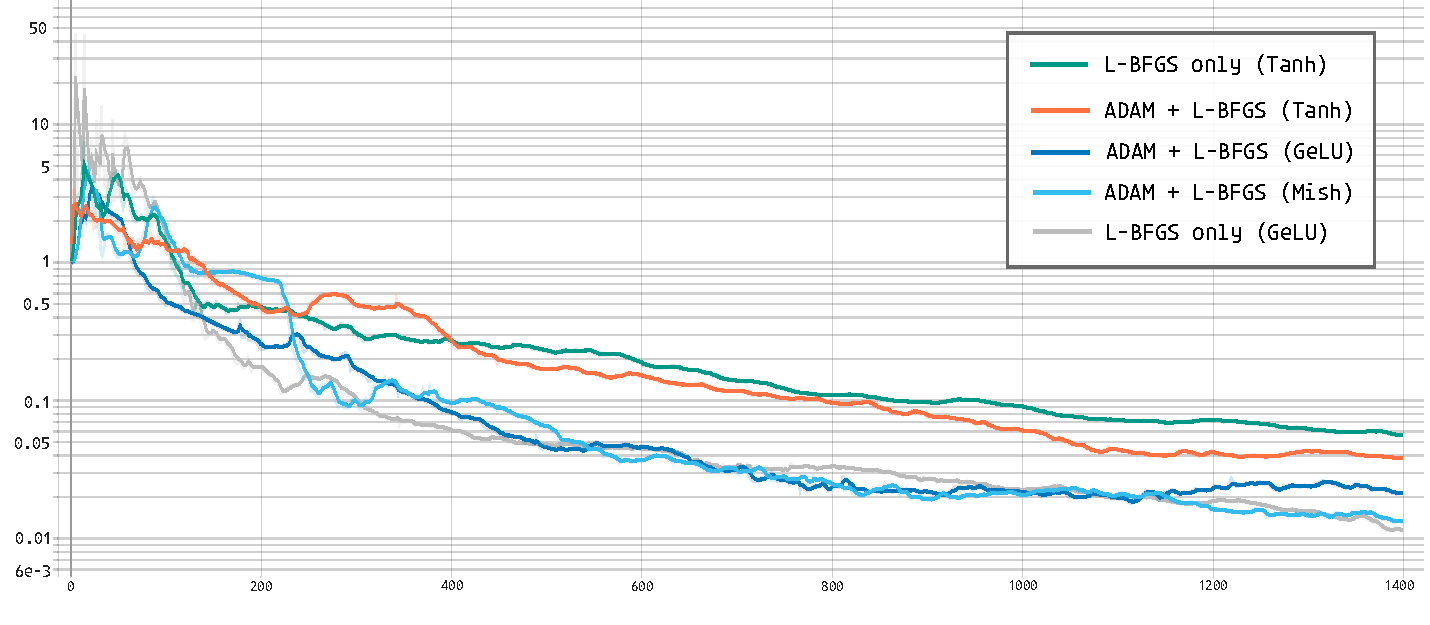
\includegraphics[width=0.8\textwidth]{./pics/MSE_relerror.pdf}}
        \caption{The convergence speed and final error of L-BFGS only and ADAM+L-BFGS. The mix method outperforms using Tanh and Mish but GeLU does not.}
        \label{fig:al}
    \end{figure}

    This mix method outperforms when using Tanh and Mish, but not in GeLU. 
    In fact, in the GeLU scenario, when increase the number of hidden layers, neurons and training points, loss fails to converge. 
    Because the performs for L-BFGS are unstable, it is better used when the loss does not converge or converges very slowly at first, or when the neural network is complicated. 

    \subsection{Getting the result}

    Figure \ref{fig:sol} and \ref{fig:error} show the prediction and error of this equation with hyper-parameters in Table \ref{table:hp1}.
    
    \begin{figure}[htb!]
        \makebox[\textwidth][c]{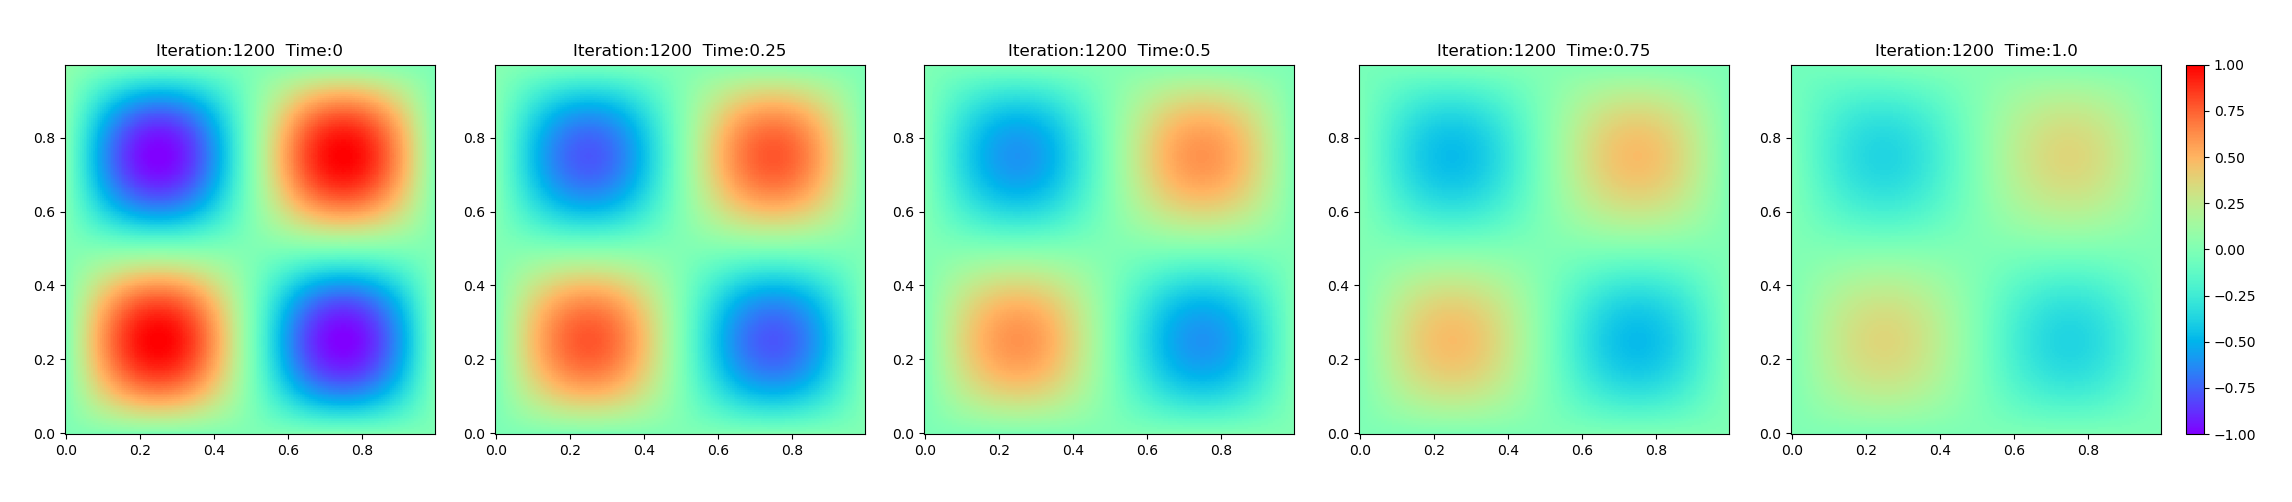
\includegraphics[width=0.9\textwidth]{./pics/sol.png}}
        \caption{The solution at $T=$ 0, 0.25, 0.5, .75 and 1.}
        \label{fig:sol}
    \end{figure}

    \begin{figure}[ht!]
        \makebox[\textwidth][c]{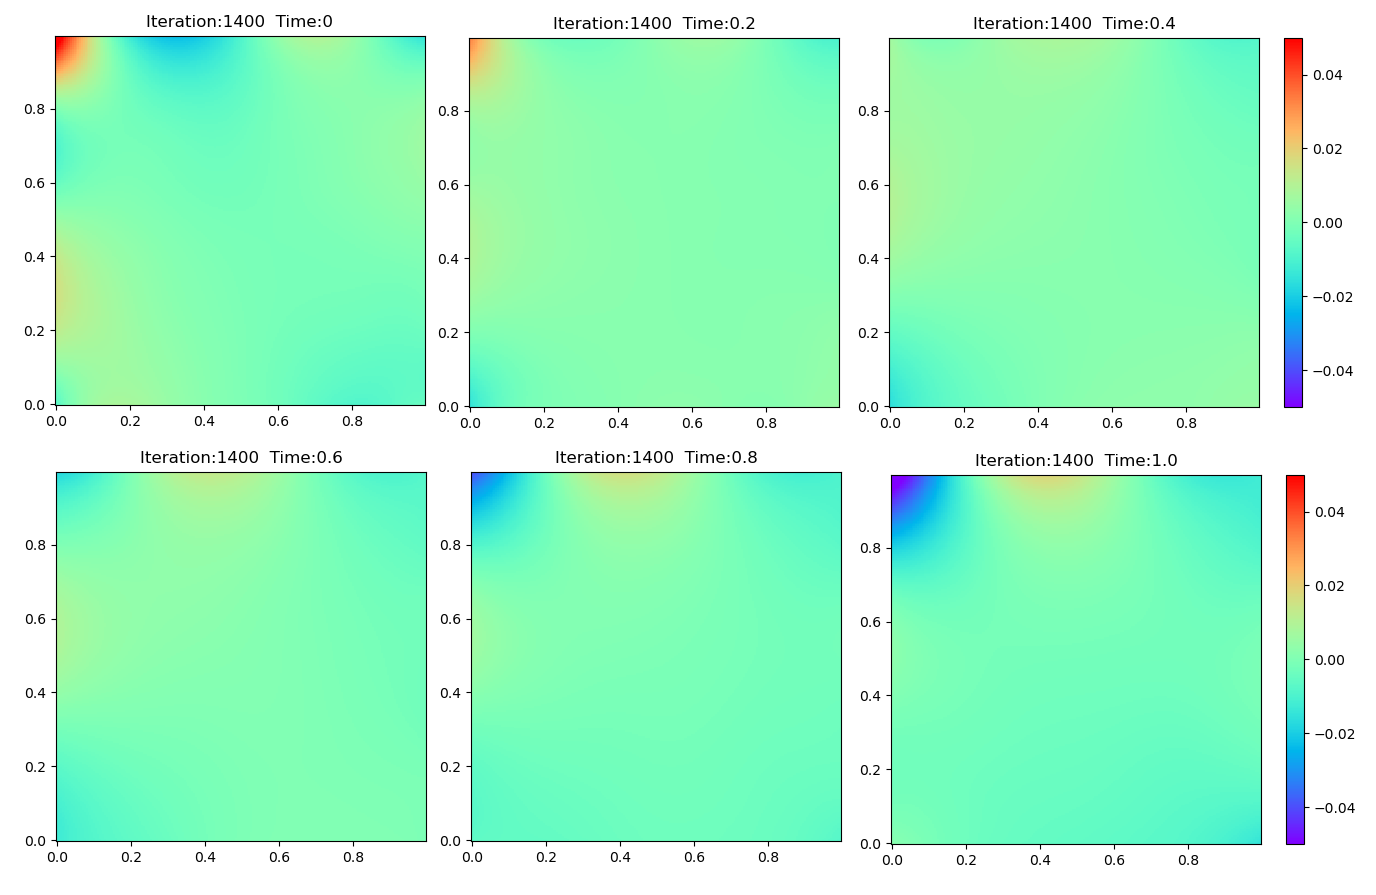
\includegraphics[width=0.9\textwidth]{./pics/error.png}}
        \caption{The error at $T=$ 0, 0.25, 0.5, .75 and 1.}
        \label{fig:error}
    \end{figure}


    Figure \ref{fig:relerrorwitht} shows the change of relative error from $T=0$ to 1. 

    \begin{figure}[ht!]
        \makebox[\textwidth][c]{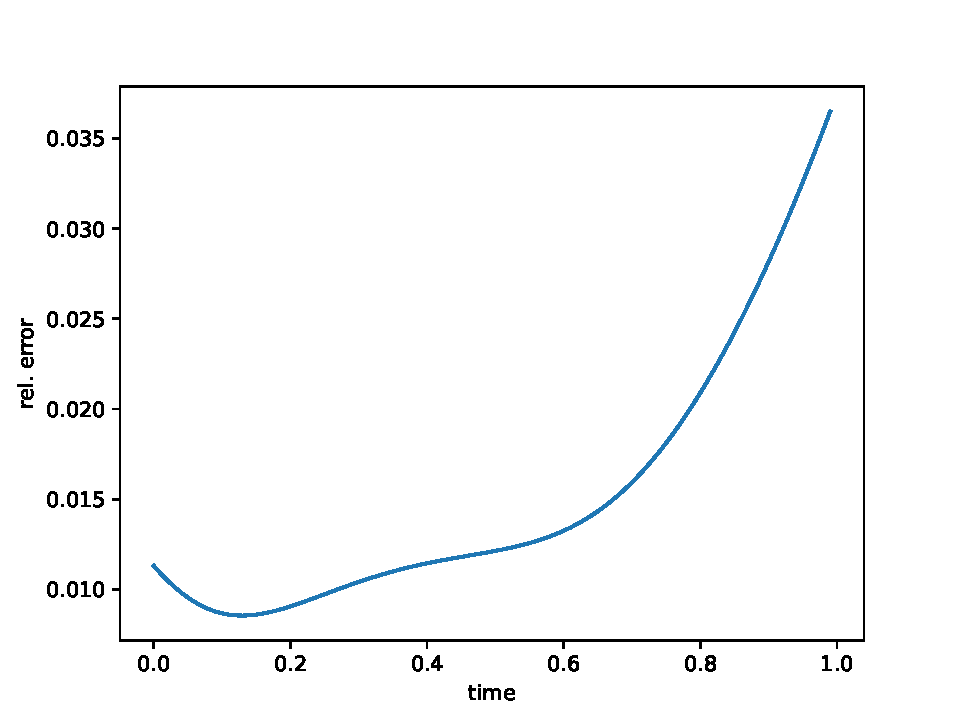
\includegraphics[width=0.65\textwidth]{./pics/rel_error_with_t.pdf}}
        \caption{Relative error from $T=0$ to 1.}
        \label{fig:relerrorwitht}
    \end{figure}

    \subsection{Investigation of Hyper-parameters}

    
    \begin{thebibliography}{9}
        \bibitem{LHS}   Zong, Yifei, QiZhi He, and Alexandre M. Tartakovsky. ``Physics-Informed Neural Network Method for Parabolic Differential Equations with Sharply Perturbed Initial Conditions." arXiv preprint arXiv:2208.08635 (2022).
    \end{thebibliography}

\end{document}